\newpage
\hypertarget{checkCard tex}{}
\subsection{Implementing check}
\texHeader
 
\begin{itemize}
   
\item[$\blacktriangleright$] In this SDM, the guess assertion, card promotion, and card penalisation must each be implemented as patterns. Given that every
action is determined a the result of a conditional statement, we can't use a simple control flow. We need an \emph{if/else} construct!

\item[$\blacktriangleright$] In the \texttt{check} declaration, create the basic \emph{if/else} construct with three patterns, as illustrated in
Fig.~\ref{fig:checkDec}. The type completion feature includes a template for this.

\vspace{0.5cm}

\begin{figure}[htbp]
\begin{center}
  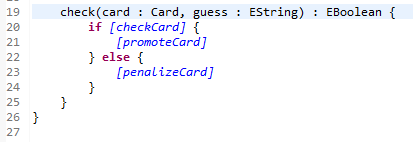
\includegraphics[width=0.65\textwidth]{eclipse_checkCardMethod}
  \caption{An if/else construct in \texttt{check}}
  \label{fig:checkDec}
\end{center}
\end{figure} 

\item[$\blacktriangleright$] Upon saving, you should again encounter some problems. Use the ``Quick Fix'' wizard to generate the pattern files. Your package
explorer should now resemble Fig.~\ref{fig:checkPatternsExplorer}.

\begin{figure}[htbp]
\begin{center}
  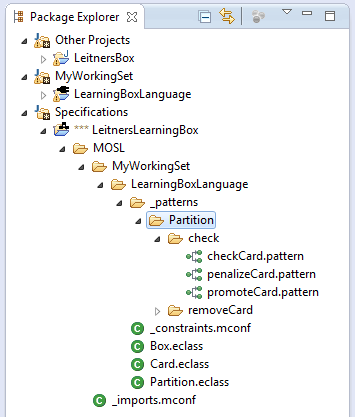
\includegraphics[width=0.55\textwidth]{eclipse_checkPackageExplorer}
  \caption{The created pattern files}
  \label{fig:checkPatternsExplorer}
\end{center}
\end{figure} 

\item[$\blacktriangleright$] Open the \texttt{checkCard} pattern. What do we need in order to validate the user's guess? Given that \texttt{guess} is a
parameter and not an object in the metamodel, the only variable we need to create is a bounded \texttt{card}. Then we'll need to specify an \emph{attribute constraint} in this variable to compare
\texttt{card} and \texttt{guess}. Attribute constraints have similar operators as Java comparators so to equate the values, we'll want to use \texttt{==}.

\item[$\blacktriangleright$] To access the \texttt{back} attribute and compare it to the parameter, simply write: 
\syntax{card.back == \$guess}
Accessing object attributes follow the tradtional \texttt{.} operator while the \texttt{\$} symbol is required to retrieve parameter values. Your completed
attribute constraint and \texttt{checkCard} pattern should now resemble Fig.~\ref{fig:checkPattern}.

\begin{figure}[htbp]
\begin{center}
  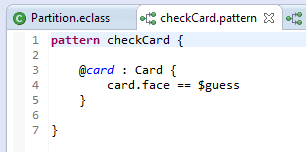
\includegraphics[width=0.5\textwidth]{eclipse_checkPattern}
  \caption{One rule for \texttt{checkCard}}
  \label{fig:checkPattern}
\end{center}
\end{figure} 

\clearpage

\item[$\blacktriangleright$] Now lets develop the \texttt{promoteCard} pattern. It requires three variables - the card, the current partition, and the partition
the card will move to. Your workspace should resemble Fig.~\ref{fig:promoteCardPattern}.

\begin{figure}[htbp]
\begin{center}
  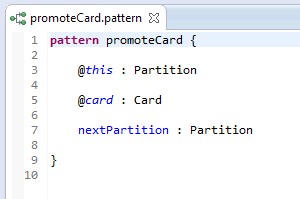
\includegraphics[width=0.5\textwidth]{eclipse_promoteCardPattern}
  \caption{Promoting a card}
  \label{fig:promoteCardPattern}
\end{center}
\end{figure} 

\item[$\blacktriangleright$] Given that \texttt{this} is bound while \texttt{next} is free, we need to establish the reference between this and the
partition, so that the card will move to the correct place. Create a simple reference from \texttt{next} to its target \texttt{nextPartition}. Your file should
now resemble Fig.~\ref{fig:promoteThisRule}.

\vspace{0.5cm}

\begin{figure}[htbp]
\begin{center}
  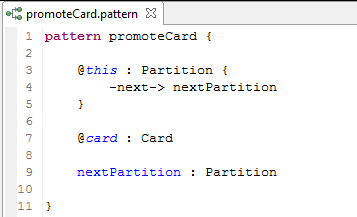
\includegraphics[width=0.5\textwidth]{eclipse_promoteCardThisRule}
  \caption{The \texttt{@this} object variable}
  \label{fig:promoteThisRule}
\end{center}
\end{figure} 

\item[$\blacktriangleright$] Finally, lets create and delete the \texttt{cardContainer} references in \texttt{card}. Make a simple destruction reference to
\texttt{this}, and a simple creation reference to \texttt{nextPartition}.\footnote{There are several different ways you could have implemented this movement, such as having a
creation reference in \texttt{nextPartition}} Your pattern is now complete, and should resemble Fig.~\ref{fig:completedPromote}.

\begin{figure}[htbp]
\begin{center}
  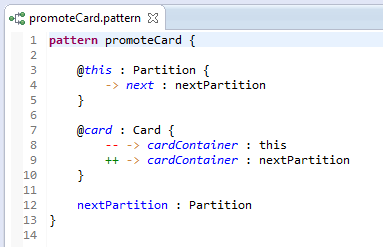
\includegraphics[width=0.6\textwidth]{eclipse_promoteCardCompleted}
  \caption{The finished \texttt{promoteCard} pattern}
  \label{fig:completedPromote}
\end{center}
\end{figure} 

\item[$\blacktriangleright$] Compare the differences between the \texttt{promoteCard} and \texttt{penalizeCard} concepts. They both do the exact same thing,
except the destination partition is slightly different. Knowing this, try to complete \texttt{penalizeCard} entirely on your own. Your workspace should come to
resemble Fig.~\ref{fig:completedPatterns}.

\begin{figure}[htbp]
\begin{center}
  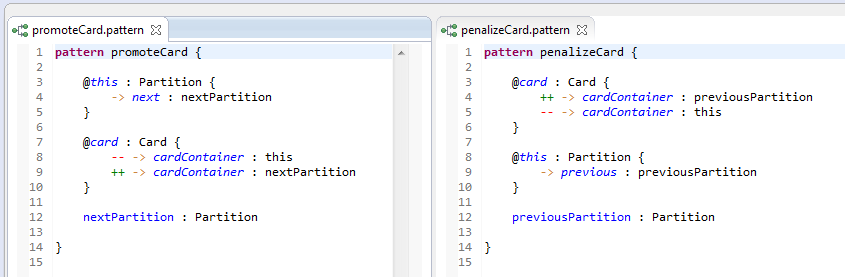
\includegraphics[width=\textwidth]{eclipse_movementPatternsCompleted}
  \caption{The finished movement patterns}
  \label{fig:completedPatterns}
\end{center}
\end{figure}


\item[$\blacktriangleright$] Did you notice that the order of the \texttt{this} and \texttt{card} object variables were reversed in our images?
Overall, for simple transformations like this, it doesn't matter in which order objects are created, or references changed in patterns. Everything just needs to
be correctly declared.

\item[$\blacktriangleright$] We nearly forgot to complete the control flow! We have specified the assertion and movements, but we haven't returned any
\texttt{EBoolean} results as the method requires. If the card was promoted, the guess was successful, so return \texttt{true} beneath \texttt{[promoteCard]}. If
it was penalized, the guess was \texttt{false}. Your \texttt{partition} EClass should now include Fig.\ref{fig:finalMethod}.

\vspace{0.5cm}

\begin{figure}[htbp]
\begin{center}
  \includegraphics[width=0.7\textwidth]{eclipse_checkMethodFinal}
  \caption{Completed control flow for \texttt{check}}
  \label{fig:finalMethod}
\end{center}
\end{figure}

\item[$\blacktriangleright$] Save and build your metamodel, then try viewing the changes in ``PartitionImpl.Java'' under \texttt{check}. You'll be able to
see the if/else construct, as well as the link manipulations. 

\item[$\blacktriangleright$] Great job! You have just implemented a new kind of control flow and created two patterns that transform cards.
To see how this SDM is implemented visually, check out Fig.~\ref{fig:sdm_check_finish} for the control flow, and Figs.~\ref{fig:sdm_check_complete_activity_node} and
\ref{fig:sdm_check_complete_penalize} for the movement patterns, all in the previous section.

\end{itemize}
 